\documentclass[12pt, a4paper, oneside]{article}
\usepackage{amsmath, amsthm, amssymb, bm, graphicx, hyperref, mathrsfs}
\usepackage{graphicx}

\title{\textbf{Assignment\#1 CS305 Fall 2023}}
\author{Ben Chen(12212231)}
\date{\today}
\linespread{1.23}
\newcounter{problemname}
\newenvironment{problem}{\stepcounter{problemname}\par\noindent\textsc{Problem \arabic{problemname}. }}{\\\par}
\newenvironment{solution}{\par\noindent\textsc{Solution. }}{\\\par}
\newenvironment{note}{\par\noindent\textsc{Note of Problem \arabic{problemname}. }}{\\\par}

\begin{document}

\maketitle

\begin{problem}
    Explain the five-layer Internet protocol stack.
\end{problem}

\begin{solution}
    The five layers of Internet protocol are(from top to bottom):
    \begin{minipage}[t]{1.0\textwidth}
        \begin{itemize}
            \item Application\newline
                Application layer is applied to support network applications such as file transportation and email exchange etc.\newline
                Typical protocols: HTTP, IMAP, FTP and Modbus.
            \item Transport\newline
                Transport layer provides process-process data transfer. It can segment the data stream and relieving congestion.\newline
                Typical protocols: TCP, UDP and RDP.
            \item Network\newline
                Network layer can routes the datagram from source to destination and switch connections through nodes in the network.\newline
                Typical protocols: IPv4/IPv6, ICMP and DDP.
            \item Link\newline
                Link layer ensure reliable data transfer between adjacent nodes by controlling the data flow.\newline
                Typical protocols: Ethernet, IEEE 802.11 and ARP.
        \end{itemize}
    \end{minipage}
    \newpage
    \begin{minipage}{1.0\textwidth}
        \begin{itemize}
            \item Physical\newline
                Physical layer deals with the data physically through wires, microwave or anything else.\newline
                Typical protocols: Bluetooth, USB and DSL.
        \end{itemize}
    \end{minipage}
\end{solution}

\begin{problem}
    What type of application is TCP/UDP better suited for? Give some application examples.
\end{problem}

\begin{solution}
    \textbf{a)} TCP is a connect-oriented and reliable protocol and therefore, is used in situations where it's necessary that all data being sent by one device is received by another completely intact. But it's less efficient. Thus, it can be used in applications like website(HTTP/HTTPS), email(SMTP), file transportation(FTP) and Telnet etc.\newline
    \textbf{b)} UDP is a datagram-oriented protocol. It's used for situations where mild data loss is acceptable and speed is a critical, like livestream and online gaming. Additionally, UDP is connectionless and can be applied in broadcasting. It has typical examples such as DNS and NTP.
\end{solution}

\begin{problem}
    A packet of $L$ bits is sent through a $K$-hops path and each link has a transmission rate of $R$ bps, 
    and the propagation delay is $d$ for each hop. 
    \textbf{a)} In a packet switching network, suppose there's no nodal processing delay and queuing delay. What is the end-to-end delay? 
    \textbf{b)} In a circuit switching network, suppose the circuit setup needs $\tau$ seconds and links use FDM where the associated frequency band is divided into F subbands. What's the end-to-end delay?
    \textbf{c)} In a packet switching network, given that $L = 100 \textit{bits}$, $K = 2$, $R = 20 \textit{Mbps}$, $d = 10\mu\textit{s}$ and nodal processing delay is $5\mu\textit{s}$, and suppose there're two packets sent. What's the time required?
\end{problem}

\begin{solution}
    \textbf{a)} The nodal delay is
    \begin{equation*}
        d_{\text{nodal}} = d_{\text{trans}} + d_{\text{prop}} = \frac{L}{R} + d
    \end{equation*}
    Thus, the end-to-end delay is
    \begin{equation*}
        d_{\text{end-to-end}} = K(\frac{L}{R} + d)
    \end{equation*}
    \textbf{b)} The end-to-end delay of circuit switching network is
    \begin{align*}
        d_{\text{end-to-end}} &= d_{\text{setup}} + d_{\text{trans}} + Kd_{\text{prop}} \\
                              &= \tau + L \cdot \frac{F}{R} + Kd
    \end{align*}
    \textbf{c)} The time required is mainly decided by the second packets, so the total queuing delay of second packet is
    \begin{equation*}
        d_{\text{queue}} = d_{\text{proc}}
    \end{equation*}
    Thus, the total delay is
    \begin{align*}
        d_{\text{end-to-end}} &= (K-1)d_{\text{proc}} + Kd_{\text{trans}} + Kd_{\text{prop}} + d_{\text{queue}} \\
                              &= 2\cdot5\mu\textit{s} + 2\cdot \frac{1000\textit{bits}}{20\textit{Mbps}} + 2\cdot10\mu\textit{s} \\
                              &= 130\mu\textit{s}
    \end{align*}
\end{solution}

\begin{problem}
    Consider a set of packets with a size of $10$ \textit{Mbits} and a queue, and the transmission rate is $10$ \textit{Mbits}.
    \textbf{a)} Suppose there's one packet arrival per second, what is the average queuing of these packets?
    \textbf{b)} Suppose $K$ packets arrive simultaneously every K seconds. What's the average queuing delay of these packets?
    \textbf{c)} What are the traffic intensity of the scenarios considered in (a) and (b)? Any insights?
\end{problem}

\begin{solution}
    \textbf{a)} Since
    \begin{equation*}
        \lambda = \frac{L}{R} = 1
    \end{equation*}
    the packets arrive periodically one after one, thus the queue will be empty and there's no queuing delay. The average queuing delay is zero.
    \newline\textbf{b)} For the $n$-th K packets arrive, the queuing delay is
    \begin{equation*}
        d_{\text{queue}} = (n-1)\cdot\frac{L}{R} = n-1
    \end{equation*}
    Thus, the average queuing delay is
    \begin{align*}
        \lim_{n\to\infty}d_{\text{avg}} &= \lim_{n\to\infty}\frac{\sum_{x=1}^n n-1}{n} \\
        &= \lim_{n\to\infty} \frac{n-1}{2} = \infty
    \end{align*}
    \newline\textbf{c)} Both of the scenarios has the traffic intensity $\rho = 1$. But there's difference that scenario (a) has no queuing delay while the average delay of (b) reaches infinity. That gives us that in the design of routers, it's better to send packets as separatedly as possible.
\end{solution}

\begin{problem}
    Given a message and answer the questions.
\end{problem}

\begin{solution}
    \textbf{a)} HTTP response message. Because it includes the Status Line (HTTP Version, Status Code and Status message) and Server etc.\newline
    \textbf{b)} A persistent connection, since ``Connection'' field indicates ``Keep-Alive''. Persistent connection means that the server-client's TCP connection stays for a while instead of closing after sending one response message. It's intended for sending multiple response messages with resources within a single TCP connection to reduce redundant time required by multiple TCP handshaking and DNS queries.\newline
    \textbf{c)} There's no blank line between the header and the entity.\newline
    \textbf{d)} To relieve the pressure of ISP servers, web caching servers are applied as a proxy server for the main ISP server. The main server delivers its resouces to the proxy servers and clients access the resources through them. The resources may be modified and proxy servers may not get the latest ones. Therefore, to help clients check whether the resources they got is updated or not, the proxy servers should provide with message that indicates the version of resources, which is exactly ``\textit{Last-Modified}''.\newline
\end{solution}

\begin{problem}
    Given a network topology, there're a set of objects with size of $1$ \textit{Mbits} each. Suppose the institution's computer has an average request rate of 10 requests per second, and all requests are sent to the origin servers. \textbf{a)}Derive average response time of the system. \textbf{b)} Suppose there's cache installed in the institutional LAN. Compute the hit rate $x$ that leads to an average response time that is less than 1 second.
\end{problem}

\begin{solution}
    \textbf{a)} The average response time of the system is
    \begin{align*}
        \Delta &= \frac{L}{R} = \frac{1\ \textit{Mbits}}{20\ \textit{Mbps}} = 0.05 \ \textit{seconds} \\
        d_{\text{res}} &= 2\ \textit{seconds} + \frac{0.05\ \textit{seconds}}{1-0.05\ \textit{seconds}\cdot 10} \\
                       &= 2.1\ \textit{seconds}
    \end{align*}
    \textbf{b)} After installing a cache with hit rate $x$, the expectation of average response time is
    \begin{align*}
        E(x) &= 0.1\ \textit{seconds}\cdot x + 2.1\ \textit{seconds}\cdot(1-x) \\
             &= 2.1-2x\ \textit{seconds}\ \le\ 1\ \textit{seconds} \\
        \text{Solution:}\ \ x &\ge 0.55
    \end{align*}
\end{solution}

\begin{problem}
    Suppose you're using a web browser and your local DNS server has stored the resource records. Let $RTT_0$ denote the duration between when your host sends a DNS query to the time when your local DNS server sends back the reply. On the page you visit, there's an HTML page and 12 refered objects. Let $RTT_1$ denote the round trip time between the localhost and the server. The HTML page and refered objects have a size of $L\ \textit{Mbit}$ each and the transmission rate is $R\ \textit{Mbps}$. Compute the time elapsing from the moment when clicking the link and to the moment the browser received all the times under the following connections.
\end{problem}

\begin{solution}
    \textbf{a)} The duration with non-persistent HTTP and no parallel TCP connections is
    \begin{align*}
        d = 13\cdot(RTT_0 + RTT_1 + \frac{L}{R})
    \end{align*}
    \textbf{b)} The duration with non-persistent HTTP and 4 parallel connections is 
    \begin{align*}
        d = \frac{13}{4}\cdot(RTT_0 + RTT_1 + \frac{L}{R})
    \end{align*}
    \textbf{c)} The duration with persistent HTTP is
    \begin{align*}
        d = RTT_0 + RTT_1 + 13\cdot\frac{L}{R}
    \end{align*}
\end{solution}

\begin{problem}
    Answer the questions related to HTTP and SMTP.
\end{problem}

\begin{solution}
    \textbf{a)} The differences are\newline
    \begin{minipage}[t]{1.0\textwidth}
        \begin{itemize}
            \item HTTP is mainly pull protocol, and SMTP is a push protocol similar to the POST method in HTTP.
            \item HTTP has one conversation (request and response), and SMTP has three conversations (handshaking, transfer and closure).
            \item SMTP requires message to be ASCII, while HTTP does not have the requirement.
            \item HTTP offers the option of persistent and non-persistent connection, while SMTP uses persistent connections.
            \item HTTP encapsulates each objects in one response message, while SMTP sends multiple objects in one message.
        \end{itemize}
    \end{minipage}
    \newline\newline\textbf{b)} Yes. Because mail access is basically a pull process, and client can pull its mail message through any pull protocols like HTTP.
    \newline\textbf{c)} We can place the receiver's mail server but we cannot place the sender's mail server since the port 25 is occupied by SMTP and sending process cannot complete.
\end{solution}

\begin{problem}
    Suppose I want to register a domain \textit{example.com} with a TLD server, and the hostname of my DNS server is \textit{dns.example.com}
    whose IP address is "200.200.200.31". Answer the questions.
\end{problem}

\begin{solution}
    \textbf{a)} \textit{.com} TLD server.
    \newline\textbf{b)} Type A record includes the hostname and IP address of my server, e.g. \textit{example.com} and "200.200.200.31". Type NS record includes the name of my domain and hostname of my DNS server, e.g. \textit{example.com} and \textit{dns.example.com}. Therefore, my DNS server becomes a SLD.
\end{solution}

\begin{problem}
    Consider a server distributes a file of $F = 20\textit{Gbits}$ to $N$ peers. The server has a upload rate of $u_s = 15\ \textit{Mbps}$. Each peer has a upload rate of $u\ \textit{Mbps}$ and a download rate of $d = 4\ \textit{Mbps}$. Plot the following curves with $x$-axis correspoinding to $N$ (ranging from 1 to 1000) and $y$ correspoinding to the minimum distribution time.
\end{problem}

\begin{solution}
    \textbf{a)} and \textbf{b)}
    \begin{figure}[!htbp]
        \caption{Time-N graph}
        \centering
        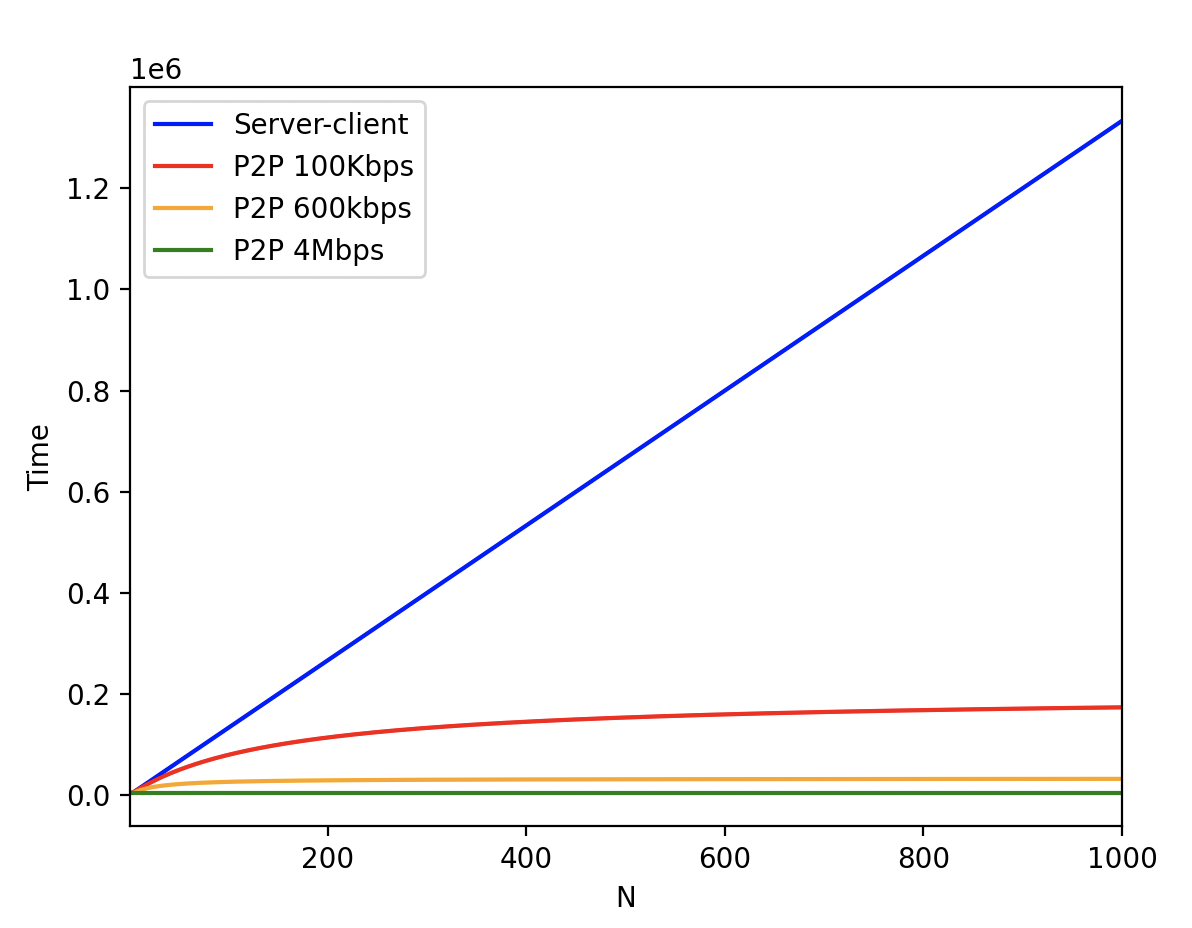
\includegraphics[width=.9\textwidth]{fig.png}
    \end{figure}
    \newline\textbf{c)} From the graph, it's obvious that P2P is better. When the number of peers $N$ increases, the distribution time of P2P $d = FN/(u_s+ Nu)$ grows slower than that of Server-client $d = NF/u_s$ because the peers are sharing the file and acting like a server, which can be considered as enlarging the bandwidth of the server. As $u$ grows, the upload time $FN/(u_s+Nu)$ keeps decreasing when the distribution time is mainly decided by it. And when $u$ and $N$ is large enough, the distribution time is bounded by the download time.
\end{solution}

\end{document}
